\documentclass[conference]{IEEEtran}
\usepackage{cite}
\usepackage{amsmath,amssymb,amsfonts}
\usepackage{algorithmic}
\usepackage{graphicx}
\usepackage{textcomp}
\usepackage{xcolor}
\usepackage{float}
\usepackage{tikz, pgfplots}
\usepackage{circuitikz}
\usepackage{booktabs}
\usepackage[english]{babel}
\usepackage[figurename=Fig.]{caption}
\usepackage[autostyle, english = american]{csquotes}

\MakeOuterQuote{"}
\def\BibTeX{{\rm B\kern-.05em{\sc i\kern-.025em b}\kern-.08em
    T\kern-.1667em\lower.7ex\hbox{E}\kern-.125emX}}

\pgfplotsset{compat=newest}

\begin{document}

\title{Autonomous Car Project\\

\author{\IEEEauthorblockN{Tevin Hendess}
\IEEEauthorblockA{\textit{Computer Engineering Department}\\
\textit{Rochester Institute of Technology}\\
Rochester, NY USA \\
twh4619@rit.edu}
\and
\IEEEauthorblockN{Adam Schultzer}
\IEEEauthorblockA{\textit{Computer Engineering Department}\\
\textit{Rochester Institute of Technology}\\
Rochester, NY USA \\
ajs1539@rit.edu}
}
}

\maketitle
\global\csname @topnum\endcsname 0
\global\csname @botnum\endcsname 0

\tikzstyle{block} = [draw, fill=white, rectangle, minimum height=2em, minimum width = 3em, align = center]
\tikzstyle{output} = [draw, fill=gray!40, rectangle, minimum height=2em, minimum width = 3em, align = center]
\tikzstyle{operator} = [draw, fill=white, rectangle, minimum height=1em, minimum width = 1em, align = center]

\begin{figure}
    \centering
    \begin{tikzpicture}
        \node (camData) [block] {Camera};
        \draw[-,thick] (camData) -- ++ (3em,0) coordinate[right] (camOut);
        \draw[->,thick] (camOut) -- ++ (3em,0) node[block,right,text width=4em] (weightedAvg) {Weighted Average};
        \draw[->,thick] (weightedAvg) -- ++ (4.5em,0) node[block,right] (pid) {PID};
        \draw[-,thick] (pid) -- ++ (0,-2em) coordinate[below] (pidOut);
        \draw[->,thick] (pidOut) -- ++ (0,-2em) node[output, below] (servo) {Servo};
        \draw[->,thick] (pidOut) -- ++ (-6em,0) -- ++ (0,-1.5em) node[block, below, text width=5em] (diffDrive) {Differential Drive};

        \draw[->,thick] (camOut) -- ++ (0,-2em) node[block, below, text width=4em] (avgBright) {Average Value};

        \draw[->,thick] ($(diffDrive.south west)!0.75!(diffDrive.south east)$) -- ++ (0, -3em) node[operator, below] (mul2) {*};
        \draw[->,thick] ($(diffDrive.south west)!0.25!(diffDrive.south east)$) -- ++ (0, -2em) node[operator, below] (mul1) {*};
        
        \draw[->,thick] ($(avgBright.south west)!0.5!(avgBright.south east)$) |- ($(mul1.south west)!0.5!(mul1.north west)$);
        \draw[->,thick] ($(avgBright.south west)!0.5!(avgBright.south east)$) |- ($(mul2.south west)!0.5!(mul2.north west)$);

        \draw[->,thick] (mul1) -- ++ (0,-3em) node[output, below, text width=3em] {Left Motor};
        \draw[->,thick] (mul2) -- ++ (0,-1.25em) -- ++ (1em,0) -- ++ (0,-0.75em) node[output, below, text width=3em] {Right Motor};

    \end{tikzpicture}
    \caption{Algorithm Flowchart}
    \label{finalAlgo}
\end{figure}

\begin{abstract}
    The Car Project of the Interfacing Digital Electronics course at the
    Rochester Institute of Technology is a well known and well respected
    part of the Computer Engineering curriculum at the university. It consists
    of using ideas developed in previous exercises to design a control system
    for a small autonomous car. This car received input only from a small
    line scan camera, making designing a control system a complex task. This
    involved finding solutions to various smaller problems, for example
    finding the center of a track piece or tuning a
    Proportional-Integral-Derivative controller to
    accurately make a turn without over- or under-shooting. Algorithms were
    designed to fulfill these requirements and were optimized to allow the
    car to make fast laps around the track. Programming the driving
    algorithm was successful, where the car was able to complete laps around
    an arbitrary track shape. In the final competition, our car placed 9th
    place out of 20 participating cars, demonstrating the prowess behind
    the theory applied to our design methodology.
\end{abstract}

\section{Introduction}
%this should be 6 paragraphs????
    This project and its associated competition component is derived from
    a similar tournament that used to take place at RIT 
    (Rochester Institute of Technology), that being the NXP
    Cup [1]. This tournament is still held in other parts of the world, but has
    been discontinued by NXP in the United States. After it's discontinuation, Texas Instruments began to provide
    microcontroller boards to RIT so that the Car Project could be continued.
    The competition component is still held every semester at RIT, including
    this Spring semester (2245).

    The rest of this paper is organized as such: After the introduction,
    Section 2 explains an overview of the materials and background information
    on the construction of the car. Section 3 introduces the main design
    methodology as well as the progression of the design over time. Section
    4 presents some experimental results during improvements as well as
    the final outcome of the RIT Car Project competition, and Section 5
    contains closing remarks.

\section{Background and Description of Components}
    Outside the controls of the car, the other important section of the lab
    was the physical construction of the car as well as the electrical
    hardware components. 

    Important to understanding the car itself is understanding the design
    constraints and development process of the vehicle and the project as a
    whole. Each team began with a set of base components which were proven to
    be functional. These components are: a vehicle base, two drive motors,
    one servo motor, a line-scan camera, two batteries, an MSP-432P4111R
    microcontroller, and a motor controller with an adapter board. 

    The total costs of all components are shown in Table \ref{tab:bom}.

    \begin{table}[h]
        \caption{Components of the Car}
        \label{tab:bom}
        \centering
        \scalebox{0.9}{ % Adjust scale if needed
        \begin{tabular}{lcr}
        \toprule
        \textbf{Part} & \textbf{Price} & \textbf{Description} \\ 
        \midrule
        Motor Driver Jumper & Provided & RPi motor driver MSP432 adapter \\ 
        Battery Charger & Provided & Charger for the two batteries \\
        Zip Ties & \$2.00 & Secures the battery to the base \\ 
        Servo Motor & \$14.99 & Futaba S3004 \\ 
        OLED Display & \$15.00 & SSD1306 \\ 
        Bluetooth Module & \$15.00 & DSD-TECH HM-10 \\ 
        TI MSP432P4111R & \$27.99 & TI MSP432P4111R microcontroller board \\
        Motor Controller & \$29.86 & MC33886 RPi Motor Driver Board \\ 
        Batteries & \$39.49 & 2x Tenergy 7.2V 3800mAh NiMH batteries \\ 
        DC Motor & \$43.90 & 2x GHM-01 12VDC 200RPM \\ 
        Vehicle Base & \$98.75 & ROB0170 \\ 
        Line Scan Camera & \$105.95 & Parallax TSL-1401 \\ 
        \bottomrule
        \end{tabular}
        }
        \end{table}

    The most basic of the provided components was a vehicle base. This was
    simply a metal frame onto which all of the electrical components could be
    attached. It contained axles and wheels with large gears which would be
    used to connect to the motors. The inclusion of gears was beneficial for
    a number of reasons. First, it allowed for the motors to be changed
    separately from the wheels and drive train itself. This isolated the two
    sections and meant that a failure in the motor didn't require replacing
    the wheels as well. The other benefit of gears was that the gear train
    allowed for an easy way to increase the torque output of the motor. The
    shaft of the motor was connected to a very small gear (12 teeth), while
    the axle for the wheels had a much larger gear (96 teeth). This meant that
    when the motor spun, the small gear would rotate eight times for every one
    revolution of the wheel. Such a gear ratio results in a much higher torque
    output on the wheel. The front wheels did not have gears as they were not
    directly powered. What they did have, however, were levers which permitted
    the wheels to turn while still spinning. This is the mechanism that the
    servo was connected to. The other notable parts of the base included
    numerous mounting points which allowed for the motors, servo, and
    electrical boards to be securely attached. The base also had a foam bumper
    in the front to avoid any shock to the circuitry if the car hit something.
    
    This frame was originally used for a similar competition which utilized
    control boards from a different manufacturer. The benefit of the frame's
    design is that it is modular, so the older boards could easily be removed
    and replaced with ones which were, at the time, still widely supported and
    available.

    The two drive motors were less complicated and simply required PWM signals
    to control their speed and power. These signals were programmed into the
    main microcontroller and then passed to the motor controller board to be
    properly translated into voltage values for the motors to understand. The
    two motors were controlled independently to allow for differential
    driving. Including this meant that when turning, the motor on the same
    side as the turn would rotate backwards, similar to how a tank would spin
    by driving its treads in opposite directions. Such functionality was
    incredibly useful as it greatly decreased the turning radius required for
    the car to navigate corners. This would not have been possible without
    independent control of the motors.

    The servo motor was the main method by which the car turned and followed
    the track, as opposed to differential drive which was only a supporting
    feature and could not turn the entire car on its own. By sending a
    position to the servo, the front wheels could be commanded into any angle.
    It was imperative that the servo be fast enough to switch continuously
    between different turning directions to get past the "snake" parts of the
    course. The holding power was also important as the servo would have to be
    able to resist the force from the track as the wheels turned and held
    through the car's high-speed maneuvering.

    The line-scan camera is the only external sensor on the car and is what
    gives the vehicle its autonomous capability. When pointed at a section of
    track (designed with two black lines surrounding a solid white center),
    the camera outputs a single 128 bit line of information about the current
    light level at each point. A sample output from the camera is shown in
    Fig. \ref{fig:camera_graph}. When viewing an image with clear contrast
    like that of the track pieces, the camera can be used to get a clear idea
    of where the edges are. The bottom graph in Fig. \ref{fig:camera_graph}
    labeled "Binary Conversion" is what the analog to digital convertor (ADC)
    on the microcontroller outputs and was originally used for controlling the
    car. At the last minute, the design shifted to use the "Smoothed Voltage"
    information instead.

    The batteries provided the electrical power for the motors, servo, camera,
    and controlling circuitry on the car. While relatively simple devices, the
    voltage level of the batteries could have a measurable impact on the
    performance of the car. While rated for 7.6 volts, the batteries could
    range from anywhere between about 7V to nearly 8V5 depending on the charge
    level. The car's motors would perform better at higher voltages, so care
    was taken to ensure that the batteries were nearly fully charged before
    important tests and that any tuning was done at a known voltage. Tuning
    values for voltages which wouldn't end up being used in the race would
    have been a waste of time.
    
    The motor controller and MSP432 are where all of the electrical signals
    were generated and contained the program which tied everything together.
    The input from the camera provided the controller with knowledge of the
    track ahead. With this information and control algorithms, it would then
    decide where the front wheels needed to turn and in what direction and
    speed the back tires had to spin. This information was sent to the motor
    controller board which then translated the commands into PWM control
    signals which would affect the required outcome on the drivetrain. The
    motor controller was also responsible for stepping down the voltage from
    the battery to a level that the MSP432 was able to run at.

    All of these components combined to form a vehicle which could take in
    information about the world around it, make decisions based on that
    information, and then execute an action. It was important, however, to
    ensure that each component was working as expected before serious effort
    could be devoted to tuning anything. To this end, the milestones focused
    on verifying the hardware, proving line-following code, testing turns and
    intersections, and finally implementing PID control and variable speed.
    At each step in this process, the challenges became more and more complex.
    By the time the final milestone was completed, however, the only work left
    was tuning the control values to the exact lighting conditions of the
    competition space. There were also some additional bonus features which
    could be added later.

    Because of how the milestones were laid out, passing one step meant that
    completing the next step would be entirely dependent on new code added
    rather than the possibility that something earlier on was broken. For
    example, testing all of the hardware to start off ensured that if the car
    randomly drove to the left, it was likely a result of the code powering
    the right motor too strongly and not because the servo had random
    twitches. Of course, some problems with hardware still arose, but any
    early ones were caught through the milestone testing.

    As a final step once the car was running, additional features could be
    added to improve functionality, prepare for extra obstacles, or gain bonus
    points. Functionality improvements included the aforementioned
    differential drive which reduced turning radii. Additionally, some time
    was devoted to preparing for the possibility that a tunnel piece would be
    added to the track. Unlike the swiggles or ramp, the tunnel altered the
    light level on the track and presented a very formidable obstacle. While
    some brainstorming was done as to how this impact could be mitigated, it
    was determined that the piece would be too disruptive to be introduced
    late in the development cycle and the choice was made to focus efforts
    elsewhere. As a final possibility, a "line-stopping" routine could have
    been implemented which would automatically stop the car once it had
    completed one lap. This was determined by a dashed line drawn
    perpendicularly across the starting track piece. Correct stopping
    functionality came with the bonus of one section removed from the car's
    final time. While such an offer is tantalizing, attempts to implement
    this feature were unsuccessful. The main reason for this failure was the
    difficulty of testing the line-stopping in the practice space. Because the
    pieces had to be moved and were not taped down, many gaps formed in
    between them as different teams tested their algorithms. This meant that
    there was a high likelihood of the line-stopping routine mistakenly
    stopping the car before the finish line, so it was abandoned.

    \begin{figure}[h]
        \centering
        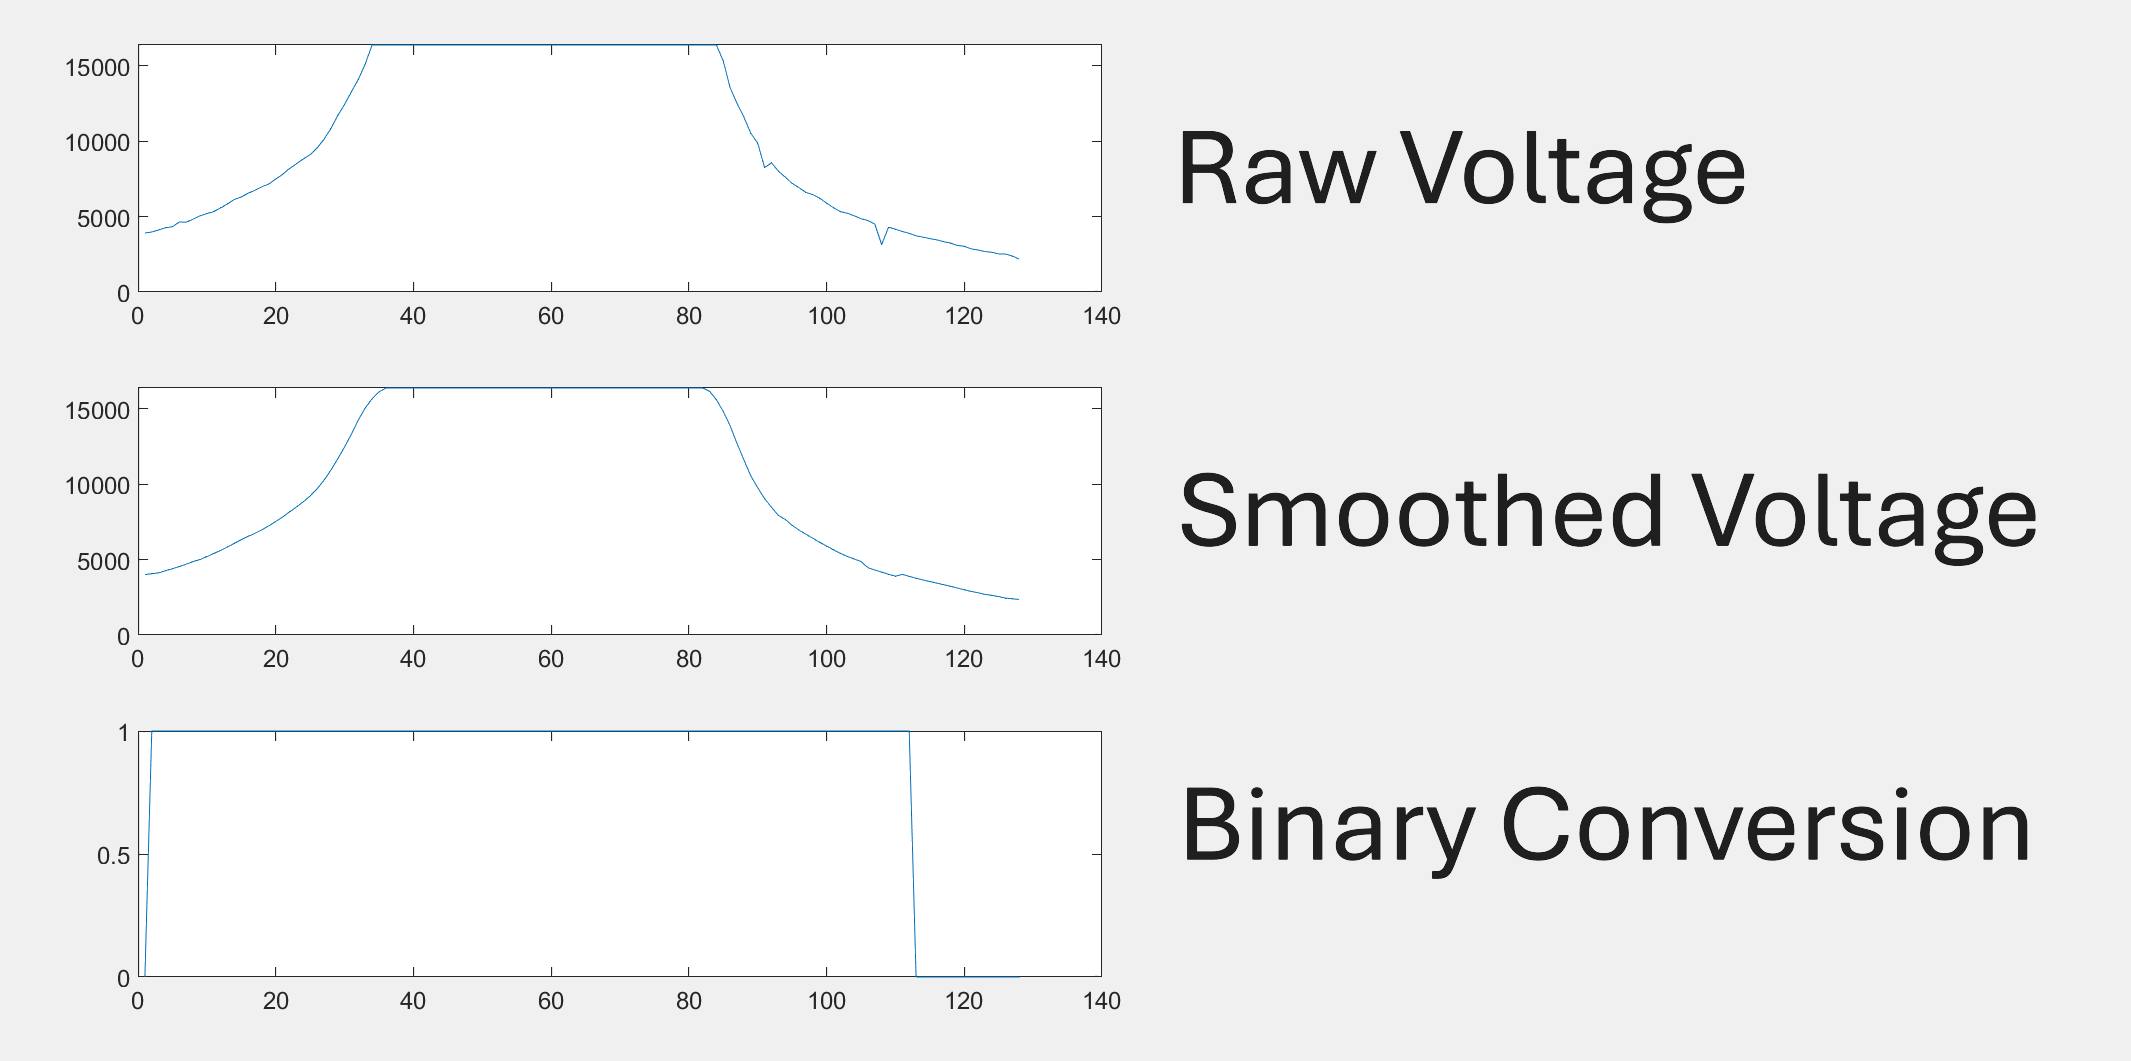
\includegraphics[width=\linewidth]{{images/part3matlab.png}}
        \caption{MatLab Graphs of Sample Camera Output}
        \label{fig:camera_graph}
    \end{figure}

\section{Design Methodology}
    The primary design challenge of allowing the car to go at a reasonable speed came in the form of algorithmic programming.
    This consisted of finding an effective way to transform the input data, a set of analog values from a line scan camera,
    to a strategic set of outputs that would drive the car in an efficient and consistent way.
    Due to the extremely limited input data at any given time, any well made algorithm would have to rely heavily on
    extracting as much information from this as possible, as well as using previous data values. 
    The algorithm for the car was created in a few iterations, moving from a more basic concept to a better fleshed out
    system for making full use of the information available.

\subsection{Basic Functionality}

\begin{figure}[h]
    \centering
    \begin{tikzpicture}
        \node (camData) [block] {Camera};
        \draw[-,thick] (camData) -- ++ (3em,0) coordinate[right] (camOut);
        \draw[->,thick] (camOut) -- ++ (3em,0) node[block,right,text width=4.1em] (weightedAvg) {Threshold Average};
        \draw[->,thick] (weightedAvg) -- ++ (4.5em,0) node[block,right] (pid) {PID};
        \draw[-,thick] (pid) -- ++ (0,-2em) coordinate[below] (pidOut);
        \draw[->,thick] (pidOut) -- ++ (0,-2em) node[output, below] (servo) {Servo};

        \node (speedSet) [block, yshift=-3em, xshift=4em] {Set Speed};

        \draw[->,thick] ($(speedSet.south west)!0.1!(speedSet.south east)$) -- ++ (0,-3em) node[output, below, text width=3em] {Left Motor};
        \draw[->,thick] ($(speedSet.south west)!0.9!(speedSet.south east)$) -- ++ (0,-3em) node[output, below, text width=3em] {Right Motor};

    \end{tikzpicture}
    \caption{Basic Algorithm Flowchart}
    \label{firstAlgo}
\end{figure}

    The first iteration of the overall algorithm used two main systems for transforming input data to output values. Firstly,
    and perhaps more importantly, the pixels in the data needed to be broadly classified as either ``track pixels'' or ``carpet pixels.''
    The easiest, and most obvious way of doing this, was to simply threshold the camera data into data that was above a certain brightness or below it.
    This was the initial implementation, and after tuning the brightness threshold value, it was quite effective at getting a good enough idea of
    what before it was track and what was the carpet.
    After the pixels were decided as either track or carpet pixels, the index of all track pixels were averaged together to get a reasonable guess
    for the center of the track.
    This system was incredibly efficient, as it only required a single comparison and addition operation for each of the 128 pixels from the camera.
    This initial system was remarkably effective when properly tuned, and was not changed until significantly later in the design process.
    Carpet stopping also followed as a direct consequence of this algorithm. Since having no track pixels would leave an undefined center, this edge
    case was simply tied to stopping the drive motors, effectively implementing carpet stopping.

    From this process, the location of the center of the track was reported as an offset from the center index of 64.
    At this point in the design process, this was reported as an integer to prevent the overhead of floating-point operations on the lower-end hardware
    of the MSP432.
    However, it was later realized that the MSP432, which is based around the ARM Cortex-M4, has dedicated floating-point hardware, so floating-point numbers were later used.
    Using this offset from center, a PID loop was implemented as a proven strategy to provide feedback to the car. Initially, all three of the proportional, integral, and derivative
    components were used, however these components were changed significantly over time.

    The output of the PID loop was used to drive the servo responsible for steering the car, allowing for the car to stay cleanly within the bounds
    of the track.
    Within the implementation, a few values required specific tuning, and would not be universal to all setups.
    Particularly, the brightness threshold value, an offset applied to steering, and the motor speed would be necessary to tune in order to recreate this algorithm.
    Of course, tuning the PID values would also be necessary after the more basic parameters were tuned.

    A flowchart of this basic algorithm is shown in Fig. \ref{firstAlgo}

\subsection{Differential Steering and Variable Speed}

    The second main iteration of the design involved the addition of two large features.
    The first of these features was differential steering, or differential drive.
    This involves taking advantage of the fact that the two back wheels could be run at independent speeds, in order to make turns more effective.
    If both wheels spin at the same speed during a turn, it means that at least one of them must slip slightly in order to allow the car to turn
    according to the steering servo. By slowing the wheel that is on the inside of the turn and speeding up the wheel that is on the outside,
    they can be made to rotate more accurately to the distance that they need to rotate through. This eliminates the majority of slipping when tuned
    correctly, and allows for the possibility of drifting.
    Drifting can be useful in order to take tighter turns than would be possible with normal driving, but comes at the cost of additional slipping,
    albeit in the opposite polarity of the case without differential steering.
    The effect of the differential steering was calculated by multiplying the output of the PID by a tunable constant, with higher values allowing for
    more slipping compensation or even drifting.
    This means that the differential steering was at any given time directly proportional to the amount of steering.

    The second of the major improvements in this iteration was variable speed. This was a natural progression from differential steering, as it also
    involves changing the speed of the driving wheels, however in this case uniformly.
    The idea behind variable speed is that due to the poor input information, the most uncertain and likely for error parts of the track would be turns,
    so it would be beneficial to slow down during them in order to allow more careful movements.
    Turns are also the most likely time to lose traction due to the previously mentioned slipping, leaving them as a key point of interest in the algorithm.
    When in the design process, there were two ways of implementing variable speed that were considered. The first tied variable speed inversely to the
    PID output.
    This would mean that whenever the car starts steering, the car would slow down to match.
    However, it was decided that this partially conflicted with the implementation of differential steering.
    So, a second option was considered.
    This second option considered the variable speed to be less about turns in particular, and more as an overall confidence interval, with the logic
    being that in any case where the car should be uncertain about what to do, it slows down.
    This was determined to be a more accurate representation of what the car should ideally do, and was chosen.

    In order to implement this confidence interval, some parameter of the input data needed to be used.
    The amount of track pixels out of the total 128 pixels was determined to be a good confidence indicator.
    This metric was chosen on the basis that the less track the car sees, the closer it must be to falling off.
    This strategy worked very well, and was kept for the rest of the process.

    An updated flowchart of this version of the algorithm is shown in Fig. \ref{secondAlgo}.

    \begin{figure}[h]
        \centering
        \begin{tikzpicture}
            \node (camData) [block] {Camera};
            \draw[-,thick] (camData) -- ++ (3em,0) coordinate[right] (camOut);
            \draw[->,thick] (camOut) -- ++ (3em,0) node[block,right,text width=4.1em] (weightedAvg) {Threshold Average};
            \draw[->,thick] (weightedAvg) -- ++ (4.5em,0) node[block,right] (pid) {PID};
            \draw[-,thick] (pid) -- ++ (0,-2em) coordinate[below] (pidOut);
            \draw[->,thick] (pidOut) -- ++ (0,-2em) node[output, below] (servo) {Servo};
            \draw[->,thick] (pidOut) -- ++ (-6em,0) -- ++ (0,-1.5em) node[block, below, text width=5em] (diffDrive) {Differential Drive};
    
            \draw[->,thick] (camOut) -- ++ (0,-2em) node[block, below, text width=4em] (avgBright) {Num of Track};
    
            \draw[->,thick] ($(diffDrive.south west)!0.75!(diffDrive.south east)$) -- ++ (0, -3em) node[operator, below] (mul2) {*};
            \draw[->,thick] ($(diffDrive.south west)!0.25!(diffDrive.south east)$) -- ++ (0, -2em) node[operator, below] (mul1) {*};
            
            \draw[->,thick] ($(avgBright.south west)!0.5!(avgBright.south east)$) |- ($(mul1.south west)!0.5!(mul1.north west)$);
            \draw[->,thick] ($(avgBright.south west)!0.5!(avgBright.south east)$) |- ($(mul2.south west)!0.5!(mul2.north west)$);
    
            \draw[->,thick] (mul1) -- ++ (0,-3em) node[output, below, text width=3em] {Left Motor};
            \draw[->,thick] (mul2) -- ++ (0,-1.25em) -- ++ (1em,0) -- ++ (0,-0.75em) node[output, below, text width=3em] {Right Motor};
    
        \end{tikzpicture}
        \caption{Differential Steering and Variable Speed Flowchart}
        \label{secondAlgo}
    \end{figure}

\subsection{Lookahead and Delayed Action}
    The final iteration to be created before the day of the competition implemented what was coined ``spooky reaction from a distance,'' for lack of a more
    defined term. 
    The inspiration behind this idea was that the car would react extremely slowly to turns once the base speed of the driving motors was increased to
    a more reasonable rate.
    After a long amount of time spent tweaking the PID values within the algorithm, it was realized that while the proportional component was having a
    useful effect, the other components were lacking this. For the integral component, anything other than an extremely small value was determined to
    be detrimental to performance, and was removed from the program entirely. The derivative component, however, was having effectively zero effect
    on the steering of the car.
    Ultimately, this lack of an effect was traced to two main issues, the primary being the use of integer types instead of floating-point types.
    The integer types led to changes in the PID input coming in small, sudden bursts, rather than gradual changes necessary for derivative to be effective.
    After some deliberation about using fixed-point numbers, and then finding that the ARM Cortex-M4 has floating point hardware, most of the
    program was swapped to using floating-point. This alone however, did not solve the issue.

    Due to the nature of thresholding the pixels, much of the analog data was gone, meaning that a shift only occurred when a full pixel shifted from
    carpet to track or the reverse. What this meant was that a change would occur in the input to the PID only occasionally, leaving large amounts
    of ticks between single ticks of the derivative having any effect. A single tick of effect was drowned out by the more consistent zero effect
    in the ticks surrounding it, leading to derivative's effect being drowned out even at absurdly high values.

    In order to fix this, the only solution found was to take the derivative over a longer period of time, allowing sparse changes to have effect in the
    derivative component for longer. To do this, a tunable number of PID input values were stored in a circular buffer, with the derivative being
    calculated using the most recent and least recent values.
    This change had the desired effect of allowing the derivative component to take a leading role in driving the car through turns.

    Despite the success of this innovation, it led to a significant side effect.
    Although the derivative was newly consistently usable, it was also delayed by a significant amount of ticks due to the longer sampling period, often
    leading to the car waiting too long to turn and either leaving the track, or having to slow down significantly to compensate for a late turn.
    This, however, was able to be turned into an advantage. Since the derivative component was now acting on relatively older data, the camera attached
    to the car could be made to look further ahead on the track, and would theoretically react to changes on time when tuned properly.
    This allowed the car to have more time to collect data on an upcoming turn, and act accordingly, rather than needing to react to a turn only
    once reached.

    Furthermore, with the proper camera lookahead angle and circular buffer size for a specific delay, the car was able to react to turns before even
    reaching them, allowing tighter turns and a lower slowdown for the turns. These changes allowed for a significant improvement in lap times during
    testing, and was expected to allow superb performance once the competition was reached.

\subsection{Competition Changes}
    Despite the many improvements made to the car over time, the conditions of the real competition track nearly entirely eliminated most performance
    uplift made. The lighting of the competition track was significantly dimmer and less consistent than the practice track.
    This change, while in theory not major, impaired the vision system of the car significantly.
    As the vision had been working with the same lighting for the entire development period, no attention was paid to any type of improvement for it.
    During the general practice time in the competition area, various values, especially the threshold brightness, were modified significantly, and
    the car was able to make a few rough laps of the practice track provided.
    Unfortunately, this practice track still only covered about a third of the space, and did not provide an accurate simulation of the lighting
    simulation for the final competition track.
    
    Once the final competition track was built, some modification was done in the five minutes provided to test the cars on the final track.
    Our car failed all attempts during this five minutes, prompting last minute changes to the vision algorithm, although they would not be
    able to be tested on a track.

    During a roughly twenty minute period after these five minutes of testing, the vision system was entirely redone to preserve the analog
    data of the pixels coming from the camera.
    This change was based entirely on theory, as testing was now unavailable, but aimed to switch from averaging the index of thresholded pixels
    to a more analog system of a weighted average based on brightness.

    This first required calculating a total brightness of the input, which was also used as the new confidence interval, rather than counting
    thresholded track pixels, shown in (\ref{brightness}).
    The algorithm then followed the formula in (\ref{weightAvg}) in order to more accurately calculate the center of brightness of the line scan
    data.

    These changes are demonstrated in a flowchart of the final algorithm shown in Fig. \ref{finalAlgo}

\begin{equation}
    B = {\sum_{n=0}^{128}D_{n}}
    \label{brightness}
\end{equation}

\begin{equation}
    x_{center} = \frac{\sum_{n=0}^{128}nD_{n}}{B}
    \label{weightAvg}
\end{equation}

\section{Results and Analysis}
    In the various stages of testing involved in our design, there were significant milestones during each, which can all be discussed at length.
    During initial testing while creating the basic algorithm, the most significant result was the car simply either staying on the track or
    falling off the track, as well as carpet stopping once it had fallen off.
    Carpet stopping was an immediete success upon implementation, and stayed consistent throughout all testing.
    The beginning of testing involved mostly the tuning of parameters like the PID constants, as well as the threshold value.
    A threshold value for brightness of 11000, out of a max of 16383, was quickly settled on, and remained consistently effective throughout most testing until competition.
    In early testing, a P value of 0.15 was determined to be effective in guiding the car through the track without oscillation at a slow speed maintained with a 35\% duty cycle.
    The I value was set as low as would be allowed while still counting for the milestone that needed to be completed at the time.
    There was an attempt to tune the D value, however, as mentioned previously, it had so little effect that it ended up being set arbitrarily at 0.1.

    In testing during the development of differential steering and variable speed, the primary results that changed based on experimentation
    were if turns could be completed at a given car speed, and how tweaking the differential steering and variable speed impacted these results.
    It was found that at very high differential coefficients, the car would start drifting and taking turns extremely sharply. This, although
    visually enticing, often left to extreme oversteering to the point where the car would turn past the curve and drive off the track. A coefficient
    too low, and the car would face the same slipping issue as without differential steering. Eventually, it was found that setting the coefficient to
    slow down the inner wheel by 80\% would result in the best turns.
    As for variable speed, it was found that scaling the speed linearly with the amount of track pixels seen, with a range from 60\% speed with no
    track pixels to a maximum of 100\% for a full image of track pixels.
    These parameters resulted in an algorithm that drove at most of the final performance, although still handling turns somewhat late and poorly.
    These late turns are of course what inspired the addition of ``spooky reaction at a distance.''

    When implementing the long period derivative and lookahead camera angle, the main results that were being monitored were the quality of the turns.
    Unfortunately a major hurdle in testing came in the form of the informality of the setup.
    Track pieces at this stage were simply placed on the ground, without any sort of way of being held in place.
    This often led to cars pushing the track out of alignment, leaving dark sections between sections that could confuse the car, leading to partially inaccurate testing.
    This was an issue for the entirety of testing, but only became a significant issue due to the new abilty to look ahead by a significant amount.
    While looking a full car length ahead, a section of darkness would throw off the car substantially more for whatever reason.

    With enough readjusting, this could be managed, but slowed down testing an unfortunate amount. Eventually, a circular buffer of size 20 was decided upon, as it introduced only a small
    delay, while still allowing the derivative component of PID to be useful. A smaller circular buffer in combination with a camera pointed at the track about a car length ahead of the
    front bumper allowed the car to preemptively react to turns.
    This preemption allowed for significantly faster and more efficient turns.
    However, a new issues was observed as a result of the higher angle of the camera.
    If for whatever reason the car failed to preemptively start a turn, the car would move a bit too far into a turn, and the camera would look past the curve into only carpet, leading 
    to the car carpet stopping in the middle of a turn.
    This meant that in order for the car to consistently make turns, the preemptive turning needed to become extremely consistent, or some modification needed to be made to carpet stopping.
    Neither of these things were able to happen due to time constraints, so the camera was set to point only about three quarters of a car length in front of the front bumper, which did not
    allow for the same level of preemptive turning, but kept the performance much more consistent.

    At the actual competition, results were vastly different from both previous results and expected results. Due to the differing lighting conditions, all practice runs were very bad,
    and although yielding useful information, did not inspire confidence in the ability of the car to complete the competition track. As previously mentioned, the car struggled to
    complete unofficial practice tracks, and completely failed to make a full lap during test runs on the official competition track.
    
    This uninspiring performance led to drastic changes in the code being made, which, as previously mentioned, were not able to be tested on a track before the competition. Despite not being
    able to test on a track, the car was able to be tested on a single leftover curved track piece that was left unused due to its yellowed state. The testing done on this piece was instrumental
    during the urgent changes made during this time. While testing the new system, there were various issues that would have entirely disabled the car during the race, for example, either not moving
    at all, or turning on the motors at full speed, beyond the safe limit.
    Despite their oppositeness, both of these issues occured within the twenty minutes of changes.

    Although the car seemed theoretically able to handle the new vision system, a single curved track piece was not enough to fully test its capabilities.
    Due to the combination of the poor performance during test runs and the fact that the new vision system would be virtually untested during the competition, the team entering the car
    was extremely uncertain that it would be able to perform correctly.
    The expected behavior was within the range of driving completely off of the track or following the track poorly and getting off course.
    However, on the first attempt during the competition, the car drove extremely consistently along the track, staying very centered and even, and completed the track in 44.680 seconds.

    From this outcome, it is likely that the base speed of the car could have been increased significantly in order to have a better time. Unfortunately, it had been decreased both intentionally
    due to uncertainty, as well as unintentially as a side effect of moving to the more analog system for the confidence interval without tuning. Ultimately, the car project was a success, as even
    with a lackluster lap time, the lap was finished in entirety, without much deviation from the center of the track.

    The aspects that most contributed to the success of the car were clearly the vision system, due to the night and day difference between practice runs and the competition run, as well as the lookahead system,
    which allowed the car to stay centered even while taking turns. The differential steering likely played a part in the great turns, but it is hard to say without testing at a higher speed. In order to improve
    the car in the future, a few particular things could be improved. Namely, the car participated in the competition effectively untuned, so better tuning could almost certainly lead to a better performance.
    A particular tuning step would certainly be increasing the speed of the car, as it had a clean run, which could have involved taking more risks for a better time.
    A further way to improve the car would almost certainly be to put more time into the algorithm for ``spooking reaction at a distance.''
    The name reflects how this part of the algorithm acts slightly like a black box. 
    Although it is clear why it works, it is not entirely clear how the tunable aspects scale or how they interact with each other, hence the lack of an ideal implementation.

\section{Comparison to Other Works}
    Autonomous vehicles have been the focus of advanced research for almost as
    long as humans have had access to computers. The vehicle developed for IDE
    was relatively simple, but at its basic level contains all of the same
    components as even the most advanced self driving cars today. A number of
    these strategies are explored in Henil Gajjar, Stavan Sanyal, and Manan
    Shah's "A comprehensive study on lane detecting autonomous car using
    computer vision".
    
    The vehicles which currently operate on the streets are made from the same
    three components as the IDE car: a controller, a computer, and a sensor.
    The car created for the class is not far behind those of the real world
    in the first two categories. The motors and servo used to control the
    propulsion are quite simple and can easily be scaled up. Similarly, while
    larger cars need more advanced computers, that is not difficult to
    implement. The main difference, therefore is the sensor.

    The IDE car is equipped with only a line-scan camera. This severely limits
    what it can see in the world. Only very clear, contrasting pathways can
    be seen at all. On top of that, lighting conditions significantly impact
    the camera's ability to tell dark from light. More advanced cars, on the
    other hand, use LiDAR and color cameras.

    More advanced sensors come with a number of advantages. They are able to
    see things beyond the road in front of them. This was a huge problem when
    there was a possibility of a tunnel being introduced into the IDE race.
    The line scan camera saw the white sides of the tunnel and interpreted 
    that as the track, so the car would drive straight into the wall. This
    problem was largely caused by the line-scan camera's inability to detect
    depth. Other sensors do not have this problem. Sensors like LiDAR are also
    able to detect people walking and other vehicles in the area.

    What is most interesting, however, is the fact that many vehicles are
    using strikingly similar algorithms to what the IDE car used. One of these
    algorithms is the Hough Line Transform explained by Open Source Computer
    Vision. Using this algorithm, straight lines on an image can be pinpointed
    and recoded as a vector of couples. Each couple is a coordinate pair which
    demarcates one edge. Determining the edges of objects from an image is
    what allows autonomous vehicles to move through the streets without
    hitting anything as they know where objects start and end. This logic is
    somewhat like what was used to keep the car within the lines of the track
    piece as the line-scan camera detected the edge of the track using the
    contrast, in a similar fashion to the Hough Transform.

    Another popular algorithm in autonomous vehicles is the Canny Edge
    Detection Model, published by John F. Canny in 1986. This algorithm is
    able to reduce a color image into only the edges of objects. Again like
    the line-scan camera, the focus of this process is on contrast. By
    removing excess information on objects and only saving their edges, the
    necessary memory and computational requirements are reduced and vehicles
    are able to navigate with relatively simple cameras.

\section{Key Challenges and What Could be Improved}

\section{Conclusion}

%COMMENTED CODE IS ALSO REQUIRED

\begin{thebibliography}{00}
    \bibitem{b1} 
    NXP (2025) \emph{NXP Intelligent Car Racing} [Online]. Available: https://nxpcup.nxp.com/
    \end{thebibliography}
%[2] https://docs.opencv.org/3.4/d9/db0/tutorial_hough_lines.html/
%[3] https://www.researchgate.net/publication/224377985_A_Computational_Approach_To_Edge_Detection
%[4] https://doi.org/10.1016/j.eswa.2023.120929

\end{document}
